\documentclass{article}

\usepackage{arxiv}

\usepackage[utf8]{inputenc} % allow utf-8 input
\usepackage[T1]{fontenc}    % use 8-bit T1 fonts
\usepackage{hyperref}       % hyperlinks
\usepackage{url}            % simple URL typesetting
\usepackage{booktabs}       % professional-quality tables
\usepackage{amsfonts}       % blackboard math symbols
\usepackage{nicefrac}       % compact symbols for 1/2, etc.
\usepackage{microtype}      % microtypography
\usepackage{lipsum}		% Can be removed after putting your text content
\usepackage{graphicx}
\usepackage[square,numbers]{natbib}
\bibliographystyle{plainnat}

\usepackage{doi}

\usepackage{cancel}
\usepackage{amsmath}
\usepackage{amsthm}
\usepackage{bm}
\usepackage{acro}
\usepackage[ruled]{algorithm2e} % load before cleveref
\usepackage[capitalise]{cleveref} 

\usepackage{mathtools} %\clap \shortintertext

\usepackage{tikz}
\usetikzlibrary{calc, angles}

\usepackage[inline]{showlabels}

\usepackage{todonotes}
\setuptodonotes{inline}

\newcommand*{\transp}[1]{#1^{\mkern-1.5mu\mathsf{T}}}
\newcommand*{\norm}[1]{\left\|#1\right\|}
\DeclareMathOperator*{\argmin}{arg~min}
\DeclareMathOperator{\interior}{int}
\DeclareMathOperator{\range}{img}
\DeclareMathOperator{\coni}{coni}
\DeclareMathOperator{\conv}{conv}
\DeclareMathOperator*{\orth}{ker}
\newcommand*{\proj}[2]{\mathfrak P_{#2}\left(#1\right)}
\newcommand*{\mul}[2]{\left\langle #1, #2 \right\rangle}
\newcommand*{\set}[1]{\left\{#1\right\}}
\newcommand*{\args}[1]{\left(#1\right)}

\newcommand*{\const}{\mathtt c}
\newcommand*{\Const}{\mathtt C}
\newcommand*{\constE}{\mathtt{c}_{\ve{e}}}

\newcommand{\RR}{\mathbb R}
\newcommand{\NN}{\mathbb N}

\newcommand*{\ve}[1]{\bm{#1}}
\newcommand*{\mat}[1]{\ve{#1}}

\newcommand*{\grad}{\ve{\nabla}\!}
\newcommand*{\jac}{\mat{\nabla}\!}

\newcommand{\iterSupP}[1]{^{(#1)}}
\newcommand{\iterSup}[1]{^{#1}}
\newcommand{\iterSubP}[1]{_{(#1)}}
\newcommand{\iterSub}[1]{_{#1}}
\newcommand{\iter}[1]{\iterSupP{#1}}

\newcommand{\xx}{x}
\newcommand{\vx}{\ve{x}}
\newcommand{\vxK}{\vx\KK}
\newcommand{\vxKp}{\vx\KKp}
\newcommand{\vxZ}{\vx\iter{0}}

\newcommand{\dCone}{\mathcal D}

\newcommand*{\vd}{\ve{d}}
\newcommand*{\vdK}{\vd\KK}
\newcommand*{\vdKp}{\vd\KKp}

\newcommand*{\vZ}{\ve{0}}

\newcommand{\kk}{k}
\newcommand{\KK}{\iterSupP\kk}
\newcommand{\kK}{\iterSubP\kk}
\newcommand{\kkn}{\kk+1}
\newcommand{\kkp}{\kk-1}
\newcommand{\KKn}{\iterSupP{\kk+1}}
\newcommand{\kKn}{\iterSubP{\kk+1}}
\newcommand{\KKp}{\iterSupP{\kk-1}}
\newcommand{\kKp}{\iterSubP{\kk-1}}

\newcommand*{\ff}{f}
\newcommand*{\vf}{\ve{\ff}}
\newcommand*{\gradf}{\grad\ff}
\newcommand*{\jacf}{\jac\vf}

\newcommand*{\lbf}{\ve{y}_{\mathrm{lb}}}
\newcommand*{\lbphi}{{y}_{\mathrm{lb}}}
\newcommand*{\slsf}{\mathcal F} %sublevelset f
\newcommand*{\lipConstf}{\mathtt{L}_{\ff}}
\newcommand*{\holderConst}{\mathtt{H}}

\newcommand{\dimIn}{N}
\newcommand{\dimOut}{K}

\newcommand{\RRin}{\mathbb R^\dimIn}
\newcommand{\RRout}{\mathbb R^\dimOut}

\newcommand*{\opt}{^*}

%\DeclareMathOperator{\int}
\newcommand{\Kone}{\mathcal K}
\newcommand*{\dualKone}{\Kone^*}
\newcommand{\leqK}{\preceq_\Kone}
\newcommand{\leK}{\prec_\Kone}
\newcommand*{\minK}{\operatorname*{min}^{\leqK}}

\newcommand{\phiC}{\varphi}
\newcommand{\func}{\mathfrak{f}}
\newcommand*{\funcX}{\func_{\vx}}
\newcommand*{\funcXK}{\func_{\vx}\KK}
\newcommand*{\funcXKp}{\func_{\vx}\KKp}

\newcommand*{\sd}{\ve{\delta}}
\newcommand*{\sdK}{\sd\KK}
\newcommand*{\sdKp}{\sd\KKp}
\newcommand*{\optVal}{\alpha}

\newcommand*{\armijoConst}{\mathtt{a}}
\newcommand*{\armijoFactor}{\mathtt{b}}
\newcommand*{\sz}{\sigma}
\newcommand*{\szK}{\sigma\iterSubP{\kk}}
\newcommand*{\szKp}{\sigma\iterSubP{\kkp}}
\newcommand*{\szKZ}{\sigma\KK\iterSub{0}}
\newcommand{\szLB}{\mathtt{M}}

\newcommand*{\suffDecConst}{\kappa_{\mathrm{sd}}}
\newcommand*{\critBound}{\varepsilon_{\mathrm{crit}}}
\DeclareAcronym{moo}{
    short={MOO},
    long={multi-objective optimization}
}

\DeclareAcronym{mop}{
    short={MOP},
    long={multi-objective optimization problem}
}

\DeclareAcronym{cg}{
    short={CG},
    long={conjugate gradient}
}

\DeclareAcronym{lhs}{
    short={LHS},
    long={left-hand side}
}

\DeclareAcronym{rhs}{
    short={RHS},
    long={right-hand side}
}

\DeclareAcronym{fr}{
    short={FR},
    long={Fletcher-Reeves}
}

\DeclareAcronym{prp}{
    short={PRP},
    long={Polak-Ribière-Polyak}
}

\theoremstyle{plain}
\newtheorem{theorem}{Theorem}
\newtheorem{lemma}[theorem]{Lemma}
\newtheorem{corollary}[theorem]{Corollary}
\theoremstyle{definition}
\newtheorem{definition}[theorem]{Definition}
\newtheorem{assumption}{Assumption}
\newtheorem*{remark*}{Remark}

\crefname{assumption}{Assumption}{Assumptions}
%\crefname{algorithm}{Algorithm}{Algorithms}

\title{
	Nonlinear Conjugate Gradient Methods with
	Guaranteed Descent for Multi-Objective Optimzation
}

\date{\today}	% Here you can change the date presented in the paper title
%\date{} 					% Or removing it

\author{%
	\href{https://orcid.org/0000-0002-3958-2277}{%
		\includegraphics[scale=0.06]{orcid.pdf}%
		\hspace{1mm}Manuel Berkemeier.%
	}\\
	Department of Computer Science\\
	Paderborn University, Germany\\
	\texttt{manuelbb@mail.uni-paderborn.de}
	\And
	\href{https://orcid.org/0000-0002-3389-793X}{%
		\includegraphics[scale=0.06]{orcid.pdf}%
		\hspace{1mm}Manuel Berkemeier.%
	}\\
	Department of Computer Science\\
	Paderborn University, Germany\\
	\texttt{sebastian.peitz@upb.de}
}%

% Uncomment to override  the `A preprint' in the header
%\renewcommand{\headeright}{Technical Report}
%\renewcommand{\undertitle}{Technical Report}
\renewcommand{\shorttitle}{\textit{arXiv} Template}

%%% Add PDF metadata to help others organize their library
%%% Once the PDF is generated, you can check the metadata with
%%% $ pdfinfo template.pdf
\hypersetup{
pdftitle={Nonlinear Conjugate Gradient Methods with Guaranteed Descent for MOO},
%pdfsubject={q-bio.NC, q-bio.QM},
pdfauthor={Manuel Berkemeier, Sebastian Peitz},
pdfkeywords={%
	Multi-Objective Optimization,
	Vector Optimization,
	Nonlinear Optimization,
	Unconstrained Optimization,
	Conjugate Gradient Method,
	Line-Search Algorithm,
}}

\begin{document}
\maketitle

% keywords can be removed
\keywords{%
	Multi-Objective Optimization
	\and
	Vector Optimization
	\and 
	Nonlinear Optimization
	\and
	Unconstrained Optimization
	\and
	Conjugate Gradient Method
	\and
	Line-Search Algorithm
}

\begin{abstract}
In this article, we present several examples of special nonlinear conjugate
gradient directions for nonlinear (non-convex) multi-objective optimization.
These directions provide a descent direction for the objectives, independent
of the line-search.
This way, we can provide an algorithm with simple, Armijo-like backtracking 
and prove convergence to a first-order critical point.
In contrast to other popular conjugate gradient methods, no Wolfe 
conditions for the step-sizes have to be satisfied.
Besides investigating the theoretical properties of the algorithm, 
we also provide numerical examples to illustrate its efficacy.
\end{abstract}

\listoftodos

\section{Introduction}
Optimization problems with two or more competing objective functions may
arise in different areas of mathematics, engineering, in the natural sciences
or in economics.
We call such problems \ac{mop} and 
\ac{moo} is concerned with finding acceptable trade-offs between the objectives of 
an \ac{mop}.
In more precise terms, optimality of our vector-valued objective function 
$\vf \colon \RRin \to \RRout$, with dimensions $\dimIn, \dimOut \in \NN$,
is determined by the partial ordering $\leK$ induced by a closed, convex, pointed cone 
$\Kone \subseteq \RRout, \interior(\Kone) \neq \emptyset$.
The solutions to the unconstrained problem
\begin{equation}
	\minK_{\vx \in \RRin}
	\begin{bmatrix}
		\ff_1(\vx)
		\\
		\vdots
		\\
		\ff_\dimOut(\vx)
	\end{bmatrix}
	\;
	=
	\;
	\minK_{\vx \in \RRin} \vf(\vx)
	\tag{MOP}
	\label{eqn:mop}
\end{equation}
are minimal with respect to $\leK$ and are called \emph{Pareto-optimal}.
That is, a point $\vx\opt\in\RRin$ is optimal, if there is no $\vx \in \RRin$ with 
$\vx \neq \vx\opt$ and 
$\vf(\vx) \leK \vf(\vx\opt) \iff \vf(\vx\opt) - \vf(\vx) \in \interior(\Kone)$.
In practical applications, one often encounters $\Kone = \RRout_{\ge 0}$.
There is a multitude of methods to solve \acp{mop}.
\todo{Elaborate and list these methods, add corresponding references.}

\subsection*{Conjugate Gradient Methods}
Originally, the \ac{cg} method is an iterative method used for the 
numerical solution of particular systems of linear equations, 
specifically those whose matrix is symmetric and positive-definite. 
The method is best suited to large-scale problems where direct methods 
are not feasible~\cite{nocedalNumericalOptimization2006}.
The linear conjugate gradient method has motivated the use of similar 
directions in iterative schemes for large-scale \emph{nonlinear} optimization
problems. 
Similarly to the linear case, the descent direction is a linear combination 
of the negative gradient and the previous direction, but the 
multipliers are different.
Today, there is a multitude of different nonlinear conjugate methods, which 
tend to be faster than the steepest descent method~\cite{nocedalNumericalOptimization2006}.

Recently,~\citet{lucambioperezNonlinearConjugateGradient2018} have adapted 
many of the popular nonlinear \ac{cg} methods to the multi-objective setting.
Their directions~\cite{%
goncalvesExtensionHagerZhang2020,%
lucambioperezNonlinearConjugateGradient2018%
} rely on strong Wolfe conditions being fulfilled.
To this end, a suitable step-size algorithm is provided~\cite{lucambioperezWolfeLineSearch2019}.
These multi-objective nonlinear \ac{cg} methods work well in experiments, 
but the line-search algorithm might require step-sizes that are 
undesirably large,
and its implementation is more involved than using simple Armijo-like backtracking.
In \cite{goncalvesStudyLiuStoreyConjugate2022}, a nonlinear \ac{cg}
method for vector optimization is proposed that works with a simple 
backtracking algorithm, but it requires estimates of the Lipschitz constants
of the objectives.

In contrast, the directions in this work satisfy a \emph{sufficient decrease}
condition by construction -- independent of the line-search.
The directions are adapted (or “translated”) from the single-objective 
setting, albeit there already is a scheme for bi-objective optimization~\cite{elboulqeExplicitThreeTermPolak}.

\section{Criticality}
Given smooth objective functions, there is necessary condition for Pareto-optimality
in~\eqref{eqn:mop} similar to Fermat's theorem in single objective optimization.
Let $\jacf(\vx) \in \RR^{\dimOut \times \dimIn}$ denote the Jacobian of $\vf$
at $\vx$. 
If $\vx\opt$ is Pareto-optimal, then it is also critical, i.e.,
\begin{equation*}
	-\interior(\Kone) \cap \range(\jacf(\vx\opt)) = \emptyset.
\end{equation*}
Vice versa, if $\vx$ is not critical, then there is a \emph{descent direction}
$\ve{v} \in \RRin$, with the defining property 
$$\jacf(\vx)\cdot \ve{v} \in -\interior(\Kone).$$
For such a direction, there is some step-size bound $\bar{\sz}>0$ such that
$$
\vf(\vx + \sz \ve{v}) \leqK \vf(\vx) \qquad \forall \sz \in (0, \bar{\sz})
\quad\text{(see \cite{granadrummondSteepestDescentMethod2005})}
.
$$
\todo{Make the above proper Definition(s)?}
Adopting the notation from~\cite{%
granadrummondSteepestDescentMethod2005,%
lucambioperezNonlinearConjugateGradient2018%
},
let $\mul{\bullet}{\bullet}$ be the usual inner product and 
%$C \subseteq \dualKone \setminus \{\vZ\}$ be a generating subset of
$$\dualKone = 
	\{
		\ve{w}\in \RRout: \mul{\ve{w}}{\ve{y}} \ge 0 
		\; \forall \ve{y}\in \Kone
	\}
,$$
the dual cone of $\Kone$.
Further, let $C \subset \dualKone\setminus \{\vZ\}$ be a compact set generating 
$\dualKone$ as its conical hull: 
$\coni(C) = \dualKone.$
Then, the map 
$$
\phiC \colon \RRout \to \RR, 
\ve{y}\mapsto 
	\sup_{\ve w \in C}\mul{\ve{y}}{\ve{w}}
	= \max_{\ve w \in C}\mul{\ve{y}}{\ve{w}}
$$
allows for a characterization of $-\Kone$ and $-\interior(\Kone)$ as its
(strict) sublevel sets at $0$:
$$
\ve y \in -\Kone \Leftrightarrow \phiC(\ve y) \leq 0,
\quad
\ve y \in -\interior(\Kone) \Leftrightarrow \phiC(\ve y) < 0.
$$
This map, the support function of the dual cone, has the following properties:

\begin{theorem}[{Lemma 3.1 in \cite{granadrummondSteepestDescentMethod2005}}]%
	\label{thm:phiC_properties}
	Let $\ve{y}, \ve{y}\prime \in \RRout$.
	Then
	\begin{enumerate}
		\item $\phiC(\ve{y}+\ve{y}\prime) \le \phiC(\ve{y}) + \phiC(\ve{y}\prime)$
			and $\phiC(\ve{y})-\phiC(\ve{y}\prime) \le \phiC(\ve{y}-\ve{y}\prime)$.
		\item If $\ve y \leqK \ve{y}\prime$, then $\phiC(\ve{y}) \leq \phiC(\ve{y}\prime)$.
			If $\ve y \leK \ve{y}\prime$, then $\phiC(\ve{y}) < \phiC(\ve{y}\prime)$.
		\item $\phiC$ is Lipschitz with constant 1.
	\end{enumerate}
\end{theorem}

Furthermore, if we define $\func\colon \RRin\times\RRin \to \RR$ by
\begin{equation*}
	\func(\vx, \ve{d})
	=
		\funcX(\ve{d})
	= 
		\phiC(\jacf(\vx)\cdot\ve{d}) 
	= 
		\max_{\ve{w}\in C} \mul{\jacf(\vx)\ve{d}}{\ve{w}}
	,
\end{equation*}
then we can infer criticality from the function $\func$.

\begin{theorem}[{Lemma 3.3 in \cite{granadrummondSteepestDescentMethod2005}}]%
	\label{thm:criticality_properties}
	Suppose $\vf$ is continuously differentiable.
	Consider the following optimization problem:
	\begin{equation}
		\min_{\ve{d}\in \RRin} 
			\funcX(\ve{d}) + \frac{1}{2}\norm{\ve{d}}_2^2
		.
		\label{eqn:sd_problem}
	\end{equation}
	Denote the minimizer by $\sd = \sd(\vx) \in \RRin$ and 
	the optimal value by $\optVal = \optVal(\vx) \in \RR$.
	\begin{enumerate}
		\item If $\vx$ is critical, then $\sd = \vZ$ and $\optVal = 0$.
		\item If $\vx$ is \emph{not} critical, then $\sd \neq \vZ$, $\optVal<0$
			and $\funcX(\sd) < - \frac{1}{2}\norm{\sd}^2 < 0$,
			and $\sd$ is a descent direction.
		\item The mappings $\vx \mapsto \sd(\vx), \vx \mapsto \optVal(\vx)$ are
			continuous.
	\end{enumerate}
\end{theorem}
Moreover, in \cite{granadrummondSteepestDescentMethod2005} it is shown that
$$
\optVal(\vx) = - \frac{1}{2}\norm{\sd(\vx)}^2
\quad\text{and thus}\quad
\funcX(\sd) = -\norm{\sd}^2.
$$
In the single-objective case, with $\Kone = \RRout_{\ge 0}$, the solution is 
$\sd = - \nabla \ff(\vx)$.
The problem in \eqref{eqn:sd_problem} thus generalizes the concept of 
the steepest descent direction, and we obtain a recipe for 
“translating” nonlinear \ac{cg} directions for multiple objectives.
Just as in single-objective optimization a sequence of directions 
$\ve{d}\KK\in \RRin$ 
is said to fulfill the sufficient decrease condition if there is a constant
$\suffDecConst > 0$ such that
$\mul{-\gradf(\vx\KK)}{\ve{d}\KK} \geq \suffDecConst \norm{\gradf(\vx\KK)}^2,$
we qualify them accordingly in the multi-objective case:

\begin{definition}
The directions $\set{\vdK}$ are said to have the 
\emph{sufficient decrease} property iff	
\begin{equation}
- 
	\funcXK(\ve{d}\KK) 
=
	-\phiC(\jacf(\vx\KK)\ve{d}\KK) 
\bm{\geq}
	- \suffDecConst \phiC(\jacf(\vx\KK)\sd\KK)
= 
	- \suffDecConst \funcXK(\sd\KK)
=
	\suffDecConst \norm{\sd\KK}^2.
\label{eqn:suff_dec}
\end{equation}
Should this hold independent of the line-search used to 
determine a step-size, we can say that the directions
$\set{\vdK}$ provide \emph{guaranteed} descent.
\end{definition}

\section{Algorithm}
The algorithm will be stated in a very generic manner.
That is, we do not yet give specific formulas to compute
the directions $\set{\vdK}$, but only assume them to have 
the sufficient decrease property~\eqref{eqn:suff_dec}.
Additionally, we have to determine step-sizes.
In the next subsection, we justify a simple backtracking
procedure.

\subsection{(Modified) Armijo Stepsize}
Let $\ve{d}\in \RRin$ be a descent direction for $\vf$ at $\vx$ and let $\ve{e}\in \Kone$
be a vector such that 
\begin{equation}
0 < \constE \leq \mul{\ve{w}}{\ve{e}}\leq 1 \qquad \forall \ve{w}\in C.
\label{eqn:amidoDinarchy}
\end{equation}
Let $\armijoConst\in(0,1)$. 
The step-size $\sz > 0$ satisfies the modified Armijo condition if 
\begin{equation}
\vf(\vx + \sz\ve{d}) 
- 
\vf(\vx) 
\leqK
-
\armijoConst \sz^2 \norm{\ve{d}}^2 \ve{e}.
\label{eqn:armijo_strict}
\end{equation}

There is a suitable step-size $\sz>0$.
\begin{proof}
	Suppose there was not:
	$$
	\vf(\vx + \sz\ve{d}) 
	-
	\vf(\vx)
	+ 
	\armijoConst \sz^2 \norm{\ve{d}}^2 \ve{e}
	\notin
	-\Kone \qquad \forall \sz > 0.
	$$
	Then there is some $\ve{w}\in C$ such that for all $\sz > 0$:
	\begin{align*}
		\mul{
			\ve w
		}{
			\vf(\vx + \sz\ve{d}) 	 
			-
			\vf(\vx)
			+ 
			\armijoConst \sz^2 \norm{\ve{d}}^2 \ve{e}
		}
	&
	> 
		0
	\\
	\mul{
			\ve w
		}{
			\sz\jacf(\ve x)\ve{d}
			+ 
			\ve{R}(\sz)
			+ 
			\armijoConst \sz^2 \norm{\ve{d}}^2 \ve{e}
		}
	&
	>
		0
	\end{align*}
	Rearranging and dividing by $\sz > 0$ gives
	\begin{align}
	\mul{\ve w}{\jacf(\vx)\ve{d}}
	&>
	-
	\armijoConst \sz \norm{\ve{d}}^2 
	\mul{\ve w}{\ve{e}}
	-
	\mul{\ve w}{\frac{\ve{R}(\sz)}{\sz}}
	\nonumber
	\\
	\mul{\ve w}{\jacf(\vx)\ve{d}}
	&>
	-
	\armijoConst \sz \norm{\ve{d}}^2
	-
	\mul{\ve w}{\frac{\ve{R}(\sz)}{\sz}}
	\label{eqn:disembranglingJonty}
	\end{align}
	where, by definition of the total differential, 
	$$
	\frac{\ve{R}(\sz)}{\sz} \to \vZ \quad\text{as $\sz \to 0$ from above.}
	$$
	Because $\ve{d}$ is a descent direction, the value on the \ac{lhs}
	in~\eqref{eqn:disembranglingJonty} is 
	constant and strictly negative, while the \ac{rhs} goes to zero.
	A contradiction!
\end{proof}

A step-size satisfying~\eqref{eqn:armijo_strict} can be found by backtracking:
Let $\kk \in \NN, \vx\KK\in \RRin$ and let $\ve{d}\KK\in \RRin$ be a descent direction
of $\vf$ at $\vx\KK$. Further, let 
$\armijoFactor \in (0,1)$ and $\armijoConst \in (0,1)$ be constants and 
$\szKZ$ an initial step-size bounded below by the constant $\szLB>0$.
Take
\begin{equation}
	\szK 
	= 
		\max_{j\in \NN_0} \armijoFactor^j\szKZ
		\quad\text{such that~\eqref{eqn:armijo_strict} holds.}
\label{eqn:backtracking_stepsize}
\end{equation}

\subsection{Algorithm}
We are now in a position to state the complete algorithm
in~\cref{algo:main_algo}.

\begin{algorithm}
	\caption{Algorithm with Generic Descent Direction}%
	\label{algo:main_algo}
	\KwData{%
		$
		\dimIn \in \NN, 
		\dimOut \in \NN,
		\vf\colon \RRin\to\RRout,
		\vxZ\in \RRin,
		\armijoConst \in (0,1), \armijoFactor \in (0,1),
		\suffDecConst > 0,
		\szKZ \geq \szLB > 0.
		$
	}
	\KwResult{
		A critical point $\vx\KK$ or a sequence $\{\vx\KK\}_{\kk\in\NN_0}$, containing a critical accumulation point.
	}
	\For{$\kk \in \NN_0$}{
		\lIf{$\vxK$ is critical}{STOP}
		Compute a direction $\vdK$ satisfying~\eqref{eqn:suff_dec}\;
		Compute a step-size $\szK$ by backtracking like in~\eqref{eqn:backtracking_stepsize}\;
		Set $\vx\KKn \leftarrow \vxK + \szK \vdK$\;
	}
\end{algorithm}

In the following we continue to establish results meant to prove converge
for specific directions $\set{\vdK}$ in subsequent sections.
Of course, there is nothing to show if we stop at a critical point 
with finite termination.
We hence implicitly assume infinite sequences from now on.
For the analysis, we introduce standard assumptions:
	
\begin{assumption}\label{ass:funcs_differentiable}
	For a given initial point $\vxZ$, the function 
	$\vf\colon \RRin \to \RRout$ is defined on the set
	$$
	\slsf = \set{
		\vx \in \RRin: \vf(\vx) \leqK \vf(\vxZ)
	}.
	$$
	Furthermore, $\vf$ is continuously differentiable in an open set 
	containing $\slsf$ and its Jacobian $\jacf$ is Lipschitz continuous
	with constant $\lipConstf > 0$.
\end{assumption}

\begin{assumption}\label{ass:monotonic_seq_bounded}
	Every non-increasing sequence in $\vf(\slsf)$,
	$$
	\{\ve{y}\KK\}_{k} \subseteq \set{\vf(\vx): \vx\in \slsf},
	\quad \ve{y}\KKn \leqK \ve{y}\KK \;\forall \kk,
	$$
	is bounded below by some $\lbf\in \RRout$ as per
	$
	\lbf \leqK \ve{y}\KK
	$ for all $\kk$.
	In terms of $\phiC$, this means 
	$
	\phiC(\lbf)-\phiC(\ve{y}\KK)
	\leq 
	\phiC(\lbf - \ve{y}\KK)
	\leq 
	0
	$
	for all $k$.
\end{assumption}

\begin{lemma}%
	\label{thm:stepNorm_zero}
	Consider an algorithmic sequence $\set{(\vxK, \vdK, \szK)}_\kk$.
	Suppose~\Cref{ass:monotonic_seq_bounded} holds. 
	Then 
	\begin{equation*}
		\lim_{\kk\to \infty} \sz^2 \norm{\ve{d}_k}^2
		=
		\lim_{\kk\to \infty} \sz^2 \norm{\ve{d}_k}^2
		= 
		0.
	\end{equation*}
\end{lemma}

\begin{proof}
	The Armijo condition~\eqref{eqn:armijo_strict} holds.
%	$$
%	\armijoConst \sz^2 \norm{\vdK}^2 \ve e \leqK 
%	\vf(\vxK) - \vf(\vxK + \szK \vdK).
%	$$
	With~\cref{thm:phiC_properties} it follows that 
	\begin{align*}
	\phiC\args{
		\vf(\vxK + \szK \vdK)
	}
	-
	\phiC\args{
		\vf(\vxK)
	}
	&\le
	\phiC\args{
		\vf(\vxK + \szK \vdK)
		-
		\vf(\vxK)
	}
	\le
	\phiC\args{
	- \armijoConst \sz^2 \norm{\vdK}^2 \ve e
	}
	\\
	\Leftrightarrow\quad
	\phiC\args{
		\vf(\vxK)
	}
	-
	\phiC\args{
		\vf(\vxK + \szK \vdK)
	}
	&\ge 
	-
	\phiC\args{
	- \armijoConst \szK^2 \norm{\vdK}^2 \ve e
	}
	=
	\armijoConst \szK^2 \norm{\vdK}^2 
	\underbrace{
		\inf_{\ve{w}\in C} \mul{\ve w}{\ve e}
	}_{\geq \constE > 0}
	.
	\end{align*}
	% Since $C$ is compact, $\mul{\ve w}{\bullet}$ is linear, and 
	% $\mul{\ve w}{\ve e}>0$ for all $\ve w$,
	% $$
	% \inf_{\ve{w}\in C} \mul{\ve w}{\ve e} 
	% =
	% \min_{\ve{w}\in C}\mul{\ve{w}}{\ve{e}}
	% = 
	% \constE > 0.
	% $$
	% There is thus a positive constant $\const > 0$ 
	% with
	% $$
	% \const \szK^2 \norm{\vdK}^2
	% \leq
	% \phiC\args{
	% 	\vf(\vxK)
	% }
	% -
	% \phiC\args{
	% 	\vf(\vxK + \szK \vdK)
	% }
	% $$
	% \todo{Prepend this fact in the definition of $\ve{e}$ and mention
	% the extreme value theorem.}
	Combining all constants into $\const >0$ and summing up to $\kappa \in \NN_0$ gives 
	$$
	\const
	\sum_{\kk=0}^\kappa
	\szK^2 \norm{\vdK}^2
	\leq
	\phiC\args{
		\vf(\vxZ)
	}
	-
	\phiC\args{
		\vf(\vx\iter{\kappa + 1} + \sz\iter{\kappa + 1} \vd\iter{\kappa + 1})
	}
	$$
	Due to~\cref{ass:monotonic_seq_bounded},
	the \ac{rhs} simplifies:
	$$
	\const
	\sum_{\kk=0}^\kappa
	\szK^2 \norm{\vdK}^2
	\leq
	\phiC\args{
		\vf(\vxZ)
	}
	-
	\phiC(\lbf)
	$$
	The \ac{lhs} is a monotonically increasing sequence and bounded above.
	Due to the Monotone Convergence Theorem, it must be convergent, i.e.,
	$$\sum_{k=0}^\infty \szK^2 \norm{\vdK}^2 < \infty $$
% For parts of the convergence theory, it actually suffices to have
% \begin{equation}
% \phiC(\vf(\vx)) 
% - 
% \phiC(\vf(\vx + \sz \ve{d})) 
% \geq
% \armijoConst 
% \sz^2 \norm{\ve{d}}^2
% \phiC(\ve{e}).
% \label{eqn:modified_armijo}
% \end{equation}
% If the modified Armijo condition~\eqref{eqn:armijo_strict} is fulfilled, then this property 
% follows from~\cref{thm:criticality_properties}.
% However, the sequence generated by~\eqref{eqn:modified_armijo}
% need no longer be $\Kone$-monotonous, and we would have 
% to require a bounded set to have everything work...
% 	With~\cref{thm:phiC_properties} we get
% 	\begin{align*}
% 		\phiC\args{\armijoConst \sz^2 \norm{\vdK}^2 \ve e}
% 		&\leq
% 		\phiC\args{\vf(\vxK) - \vf(\vxK + \szK \vdK)}
% 	\end{align*}
\end{proof}

\begin{theorem}%
	\label{thm:armijoZoutendijk}
	Suppose~\cref{ass:funcs_differentiable,ass:monotonic_seq_bounded} hold
	and that the step-sizes $\szK$ in~\cref{algo:main_algo}
	satisfy~\cref{eqn:armijo_strict}.  
	Then following Zoutendijk-like condition follows:
	\begin{equation}
		\sum_{\kk \in \NN_0}
		\frac{
			\norm{\sdK}^4
		}{
			\norm{\vdK}^2
		}
		=
		\sum_{\kk \in \NN_0}
		\frac{
			\funcXK(\sdK)^2
		}{
			\norm{\vdK}^2
		}
		<
		\infty
	\end{equation}
\end{theorem}
\begin{proof}
	Let $\kk\in\NN_0$ and consider two cases.

	First, suppose $\szK\ne\szKZ$.
	Due to the backtracking procedure, the Armijo condition must be violated 
	for $\szK \armijoFactor^{-1} > \szK$.
	I.e., there is $\ve{w}\in C$ such that 
	\begin{align*}
		\mul{
			\ve w
		}{
			\vf\args{\vx + \frac{\szK}{\armijoFactor}\vdK}
			-
			\vf(\vx)
			+ 
			\armijoConst \frac{\sz^2}{\armijoFactor^2} \norm{\vdK}^2 \ve{e}
		}
	&
	> 
		0.
	\end{align*}
	It follows, that
	\begin{align*}
	-\armijoConst \frac{\sz^2}{\armijoFactor^2} \norm{\vdK}^2
	\leq
	\mul{
		\ve w
	}{
		-\armijoConst \frac{\sz^2}{\armijoFactor^2} \norm{\vdK}^2 \ve{e}
	}
	<
	\mul{
			\ve w
		}{
			\vf\args{\vx + \frac{\szK}{\armijoFactor}\vdK}
		}
		-
		\mul{
			\ve w
		}{%
			\vf(\vx)
		}.
	\end{align*}
	Applying the mean-value-theorem on the \ac{rhs}
	gives some 
	$h \in (0,1)$ with
	\begin{align*}	
		-\armijoConst \frac{\sz^2}{\armijoFactor^2} \norm{\vdK}^2
		&\leq
		\frac{\szK}{\armijoFactor}
		\mul{
			\ve{w}
		}{
			\jacf\args{\vxK + h \frac{\szK}{\armijoFactor}\vdK}\vdK
		}
		\\
		&=
		\frac{\szK}{\armijoFactor}
		\mul{
			\ve{w}
		}{
			\args{
				\jacf\args{\vxK + h \frac{\szK}{\armijoFactor}\vdK}
				-
				\jacf(\vxK)
			}\vdK
			+ 
			\jacf(\vxK)\vdK
		}
		\\
		&\leq
		\frac{\szK^2}{\armijoFactor^2}
		\lipConstf
		\norm{\ve{w}}\norm{\vdK}^2 
		+ 
		\funcXK(\vdK),
	\end{align*}
	where in the last line we have used the Cauchy-Schwarz inequality
	and the Lipschitz continuity of $\jacf$ by~\cref{ass:funcs_differentiable}.
	Because $C$ is compact, $\norm{\ve w}$ is bounded and there is a constant
	$\const > 0$ such that
	$$
	\szK\ge \const \frac{-\funcXK(\vdK)}{\norm{\vdK}^2}.
	$$
	Plugging this into the Armijo condition for $\szK$ gives
	\begin{equation}	
	\phiC(\vf(\vxK))
	-
	\phiC\args{\vf\args{\vxK}}
	\geq 
	\armijoConst
	\const
	\constE
	\frac{
		\funcXK(\vdK)^2
	}{
		\norm{\vdK}^2
	}
	\geq 
	\armijoConst
	\const
	\constE
	\suffDecConst
	\frac{
		\norm{\sdK}^4
	}{
		\norm{\vdK}^2
	}.
	\label{eqn:untuningCreatrixes}
	\end{equation}

	Now, suppose $\szK = \szKZ$.
	By definition of $\sdK$ as the minimizer of~\eqref{eqn:sd_problem}, we have
	$$
	\funcXK(\sdK) + \frac{\norm{\sdK}^2}{2}
	\leq
	\funcXK(\suffDecConst^{-1}\vdK) + \frac{\norm{\vdK}^2}{2\suffDecConst^2}
	$$
	Because $\funcXK(\suffDecConst^{-1}\vdK) \leq \funcXK(\sdK)$,
	it must hold that $\norm{\sdK}^2 \leq \dfrac{\norm{\vdK}^2}{\suffDecConst^2}$.
	Thus,
	$$
	\frac{
		\norm{\sdK}^4
	}{
		\norm{\vdK}^2
	}
	\leq
	\frac{1}{\suffDecConst^4}
	\norm{\vdK}^2
	\leq
	\frac{1}{\suffDecConst^4\armijoConst\left(\szKZ\right)^2}
	\args{
	\phiC(\vf(\vxK))
	-
	\phiC\args{\vf\args{\vxK}}
	}
	$$
	As $\szKZ \ge \szLB > 0$ for all $k$,
	we again obtain an expression
	\begin{equation}
	\bar{\const}
	\frac{
		\norm{\sdK}^4
	}{
		\norm{\vdK}^2
	}
	\leq
	\phiC(\vf(\vxK))
	-
	\phiC\args{\vf\args{\vxK}}
	\label{eqn:skiascopyNoncoital}
    \end{equation}
	for some constant $\bar{\const}>0$.

	Similarly to above,
	with~\cref{ass:monotonic_seq_bounded} we can 
	deduce convergence from~\eqref{eqn:untuningCreatrixes}
	and~\eqref{eqn:skiascopyNoncoital}:
	$$
	\sum_{\kk\in\NN_0}\frac{
		\norm{\sdK}^4
	}{
		\norm{\vdK}^2
	}
	<
	\infty.
	$$
\end{proof}

Later, the Zoutendijk property allows for a convenient 
way to prove convergence for certain direction schemes
by means of contradiction, as 
made explicit with the following corollary.
\begin{corollary}\label{thm:convergence}
	Suppose, the criticality is uniformly bounded from below via
	\begin{equation}
		\norm{\vdK} \geq \critBound > 0 
		\qquad \forall \kk\in\NN_0.
		\label{eqn:critBoundedBelow}
	\end{equation}
	If the directions $\set{\vdK}$ and 
	step-sizes are chosen so 
	that~\cref{thm:armijoZoutendijk}
	applies, \textbf{and} it additionally holds that
	$$
		\sum_{\kk\in\NN_0}
		\frac{\norm{\sdK}^4}{\norm{\vdK}^2}
		= 
		\infty
		,
	$$
	then
	$
	\liminf_{\kk \to \infty}
	\norm{\sdK} = 0.
	$
	That is, there is a subsequence of iterates $\{\vxK\}$
	converging to a Pareto-critical point.
\end{corollary}

We might refer to a subsequence converging to a 
Pareto-critical point as a \emph{critical} sequence
later on.
If the directions $\set{\vdK}$ remain bounded, then
this constitutes a special case:
\begin{corollary}%
	\label{thm:dirsBoundedConvergence}
	Suppose that~\eqref{eqn:critBoundedBelow} holds and 
	that~\cref{thm:armijoZoutendijk} applies.
	If there is a constant $\Const_{\vd} > 0$ with 
	$$
	\norm{\vdK} \leq \Const_{\vd}
	\qquad \forall \kk \in \NN_0,
	$$
	then there is a critical subsequence.
\end{corollary}

\section{Specific Directions with Guaranteed Descent}

\subsection{Two Flavors of Fletcher-Reeves}
We will show two fun variants derived from 
the single-objective scheme in~\cite{zhangGlobalConvergenceModified2006}.
The directions $\vdK$ are inspired by the
classical \ac{fr} recipe and given by
\begin{equation}
	\vdK = 
	\begin{cases}
		-\ve{g}\KK
		&\text{if $\kk=0$},
		\\
		-\theta\kK\ve{g}\KK
		+ 
		\beta\kK
		\vd\KKp
		&\text{if $\kk\geq 1$,}
	\end{cases}
	\quad
	\beta\kK
	:= 
	\frac{\norm{\ve{g}\KK}^2}{\norm{\ve{g}\KKp}^2},
	\;
	\theta\kK
	:=
	\frac{
		\mul{\vdK}{\ve{g}\KK - \ve{g}\KKp}
		}{
			\norm{\ve{g}\KK}^2
		},
		\tag{FR~SO}
		\label{eqn:frSO}
\end{equation}
where $\ve{g}\KK = \gradf(\vxK)$.

\subsubsection*{FR Restart Variant}
Unfortunately, simply replacing $-\ve{g}\KK$ 
with the multi-objective steepest descent direction
$\sdK$ from~\eqref{eqn:sd_problem} and modifying 
the product in $\theta\kK$ as per
\begin{equation}
	\tilde{\beta}\kK 
	= 
	\frac{
		\norm{\sdK}^2
	}{
		\norm{\sd\KKp}^2
	}
	=
	\frac{\funcXK(\sdK)}{\funcXKp(\sd\KKp)},
	\quad
	\tilde{\theta}\kK
	=
	\frac{
		\funcXKp(\vd\KKp)
		-
		\funcXK(\vd\KKp)
	}{
		\funcXKp(\sd\KKp)
	}
	\label{eqn:hyposulphurousTontiners}
\end{equation}
does not suffice to show the sufficient decrease property~\eqref{eqn:suff_dec}.
$\tilde{\theta}\kK$ might become negative.
This can be avoided with standard Wolfe conditions.
Or with restarts, as in the following definition:
\begin{equation}
	\vdK
	=
	\begin{cases}
		\sdK
		&\text{if $\kk = 0$},
		\\
		\theta\kK \sdK + \beta\kK \vd\KKp,
		&\text{if $\kk \geq 1$,}
	\end{cases}
	\quad
	(\theta\kK, \beta\kK)
	= 
	\begin{cases}	
		(\tilde\theta\kK, \tilde\beta\kK)
		&\text{if $\tilde\theta\kK < 0$,}
		\\
		(1, 0)
		&\text{else.}
	\end{cases}
	\tag{FR~MOI}
	\label{eqn:frMO1}
\end{equation}

\begin{theorem}
	The directions in~\eqref{eqn:frMO1}
	have the sufficient decrease property~\eqref{eqn:suff_dec}
	with $\suffDecConst = 1$.
\end{theorem}

\begin{proof}
	For $\kk=0$ and $\tilde\theta\kK$ there is nothing
	to show.
	Assume $\kk \geq 1$ and $\tilde\theta\kK \geq 0$.
	Let $\ve{w}\in C$.
	\begin{align*}
		\mul{
			\ve w
		}{
			\jacf(\vxK)
			\vdK
		}
		&=
		\mul{\ve w}{
			\jacf(\vxK)
			\args{\theta\kK\sdK + \beta\kK \vd\KKp}
		}
		\\
		&= 
		\theta\kK\mul{\ve w}{\jacf(\vxK)\sdK}
		+
		\beta\kK\mul{\ve w}{\jacf(\vxK)\vd\KKp}
		\\
		&\leq
		\theta\kK\funcXK(\sdK)
		+
		\beta\kK\funcXK(\vd\KKp)
		\\
		&\stackrel{\eqref{eqn:hyposulphurousTontiners}}=
		% \frac{
		% \args{
		% 	\funcXKp(\vd\KKp)
		% 	-
		% 	\funcXK(\vd\KKp)
		% }\funcXK(\sdK)
		% +
		% \funcXK(\sdK)\funcXK(\vd\KKp)
		% }{\funcXK(\sd\KKp)}
		% \\
		% &=
		\funcXK(\sdK)
		\frac{
			\funcXKp(\vd\KKp)
			\cancel{
			-\funcXK(\vd\KKp)
			+\funcXK(\vd\KKp)
			}
		}{\funcXKp(\sd\KKp)}
		.
	\end{align*}
	By induction $\funcXKp(\vd\KKp) \leq \funcXKp(\sd\KKp)$
	and finally
	$$
	\mul{
		\ve w
		}{
			\jacf(\vxK)
			\vdK
		}
	\leq
	\funcXK(\sdK)
	\;\forall \ve{w}\in C
	\quad\Leftrightarrow\quad
	\funcXK(\vdK) \leq \funcXK(\sdK).
	$$
\end{proof}

\begin{theorem}%
	\label{thm:frMO1convergence}
	Suppose~\cref{%
	ass:funcs_differentiable,%
	ass:monotonic_seq_bounded}
	hold and that the criticality $\norm{\sdK}$ is 
	bounded below like in~\eqref{eqn:critBoundedBelow}.
	Then the Algorithm with modified Armijo-stepsizes
	according to~\eqref{eqn:armijo_strict} and with directions defined
	by~\eqref{eqn:frMO1} generates a critical subsequence.
\end{theorem}

\begin{proof}
	Denote by $\mathcal P\subseteq \NN_0$ those iteration
	indices for which $\tilde{\theta}\kK \geq 0$ and 
	by $\mathcal N\subseteq \NN_0$ the indices with 
	$\tilde{\theta}\kK < 0$.
	
	The case $\mathcal P = \emptyset$ reduces to
	$\vdK = \sdK$ for all $\kk$ and 
	$$
	\sum_{\kk \in \NN_0}
	\frac{\norm{\sdK}^4}{\norm{\vdK}^2}
	=
	\sum_{\kk \in \NN_0}
	\norm{\sdK}^2
	\geq \sum_{\kk \in \NN_0} \critBound^2
	= 
	\infty.
	$$

	If $\mathcal P \neq \emptyset$, but still
	$|\mathcal N| = \infty$, then
	$$
	\sum_{\kk \in \mathcal N \cup \mathcal P}
	\frac{\norm{\sdK}^4}{\norm{\vdK}^2}
	=
	\underbrace{
		\sum_{\kk \in \mathcal N} \norm{\sdK}^2
	}_{=\infty}
	+
	\underbrace{
		\sum_{\kk \in \mathcal P}
		\frac{\norm{\sdK}^4}{\norm{\vdK}^2}
	}_{\geq 0}
	= \infty.
	$$

	Finally, assume that $|\mathcal P| = \infty$ and
	$|\mathcal N| < \infty$.
	Let $\kk_0$ be the maximal element in $\mathcal N$.
	For all $\kk > \kk_0$ it holds that 
	$\theta\kK = \tilde\theta\kK \geq 0$ and 
	$\beta\kK = \tilde\beta\kK \geq 0$.
	Squaring~\eqref{eqn:frMO1} for any $\kk\geq 1$
	gives
	\begin{align}
		\norm{\vdK}^2 
		&= 
		\theta\kK^2 \norm{\sdK}^2
		+
		\beta\kK^2 \norm{\vdKp}^2
		+ 
		2\theta\kK \beta\kK 
		\mul{\sdK}{\vdKp}
		\nonumber
		\shortintertext{and multiplication with $\sdK$ results in}
		\mul{\sdK}{\vdKp}
		&=
		\theta\kK
		\norm{\sdK}^2
		+ 
		\beta\kK \mul{\sdK}{\vdKp},
		\nonumber
		\shortintertext{resulting in}
		\norm{\vdK}^2
		&= 
		\beta\kK^2
		\norm{\vdKp}^2
		-
		\theta\kK^2
		\norm{\sdK}^2
		+
		2 \theta\kK 
		\mul{\sdK}{\vdK}.
		\label{eqn:ethylsBabyproofed}
	\end{align}
	As shown in~\cite{granadrummondSteepestDescentMethod2005},
	the steepest descent direction is a weighted
	sum of gradients.
	More precisely, let $\tilde C = \conv(C)$, then 
	$$
	\sdK = \transp{\jacf(\vxK)}\ve{w}^*
	\quad\text{with}\quad
	\ve{w}^* = 
	\argmin_{\ve w\in \tilde C}
	\norm{\transp{\jacf(\vxK)}\ve{w}}^2.
	$$
	Thus,
	\begin{align*}
	\mul{\sdK}{\vdK}
	&=
	-\mul{\vdK}{\transp{\jacf(\vxK)}\ve{w}^*}
	\\
	&\geq
	\min_{\ve w \in C}
	-\mul{\vdK}{\jacf(\vxK)\ve w}
	=
	-
	\max_{\ve w \in C}
	\mul{\vdK}{\transp{\jacf(\vxK)\ve w}}
	=
	- \funcXK(\vdK)
	\\
	&\geq
	-
	\funcXK(\sdK)
	\geq 0,
	\end{align*}
	where we have used the fact that it does not matter
	whether we calculate $\funcXK$ over $C$ or $\tilde C$,
	and lastly the sufficient decrease property of $\vdK$.
	It follows that
	$$
	\frac{
		2 \theta\kK 
		\mul{\sdK}{\vdK}
	}{
		\norm{\sdK}^4
	}
	=
	\frac{
		2 \theta\kK 
		\mul{\sdK}{\vdK}
	}{
		(-\funcXK(\sdK))
		(-\funcXK(\sdK))
	}
	\leq
	\frac{
		2 \theta\kK 
		\mul{\sdK}{\vdK}
	}{
		\mul{\sdK}{\vdK}
		(-\funcXK(\sdK))
	}
	= 
	\frac{2\theta\kK}{\norm{\sdK}^2}.
	$$
	Combining this with~\eqref{eqn:ethylsBabyproofed} gives
	\begin{align}
		\frac{
			\norm{\vdK}^2
		}{
			\norm{\sdK}^4
		}
		&=
		\frac{
			\beta\kK^2\norm{\vdKp}^2
		}{
			\norm{\sdK}^4
		}
		-
		\frac{
			\theta\kK^2
		}{
			\norm{\sdK}^2
		}
		+ 
		\frac{
			2\theta\kK\mul{\sdK}{\vdK}
		}{
			\norm{\sdK}^4
		}
		\nonumber
		\\
		&\leq
		\frac{
			\beta\kK^2\norm{\vdKp}^2
		}{
			\norm{\sdK}^4
		}
		-
		\frac{
			\theta\kK^2 - 2 \theta\kK
		}{
			\norm{\sdK}^2
		}
		\nonumber
		\\
		&=
		\frac{
			\beta\kK^2\norm{\vdKp}^2
		}{
			\norm{\sdK}^4
		}
		-
		\frac{
			(\theta\kK -1)^2
		}{
			\norm{\sdK}^2
		}
		+
		\frac{1}{\norm{\sdK}^2}
		\nonumber
		\\
		&\leq
		\frac{
			\beta\kK^2\norm{\vdKp}^2
		}{
			\norm{\sdK}^4
		}
		+
		\frac{1}{\norm{\sdK}^2}.
		\label{eqn:recalcitratedLinearly}
	\end{align}
	In particular, for $\kk > \kk_0$, with
	$\beta\kK = \norm{\sdK}^2 / \norm{\sdKp}^2$,
	we find
	$$
	\frac{\norm{\vdK}^2}{\norm{\sdK}^4}
	\leq
	\frac{\norm{\vdKp}^2}{\norm{\sdKp}^4}
	+ \frac{1}{\norm{\sdK}^2}
	\leq
	\frac{\norm{\vdKp}^2}{\norm{\sdKp}^4}
	+ \frac{1}{\critBound^2}.
	$$
	Recursion gives
	$$
	\frac{\norm{\vdK}^2}{\norm{\sdK}^4}
	\leq
	\frac{\norm{\vd\iter{\kk_0}}^2}{\norm{\sd\iter{\kk_0}}^4}
	+
	\sum_{i=\kk_0 + 1}^k
	\frac{1}{\critBound^2}
	=:
	\Const_0
	+
	\frac{\kk - \kk_0}{\critBound^2}
	=
	\frac{(\Const_0 \critBound^2 - \kk_0) + \kk}{\critBound^2}.
	$$
	Summation of the reciprocals results in a 
	divergent sum (because the harmonic series diverges):
	$$
	\sum_{\kk>\kk_0}
	\frac{\norm{\sdK}^4}{\norm{\vdK}^2}
	\geq 
	\sum_{\kk>\kk_0}
	\frac{
		\critBound^2
		}{
		(\Const_0 \critBound^2 - \kk_0) + \kk
	}
	= \infty.
	$$

	This concludes the proof, as~\cref{thm:convergence} applies.
\end{proof}

\subsubsection*{FR MaxiMin Variant}
The other variant based on the single-objective 
scheme~\eqref{eqn:frSO} directly exploits
the definition of $\funcXK$ as a maximization problem
over $C$.
More precisely, for $\kk \ge 1$ and $\ve{w}\in C$,
define the coefficients
% \begin{equation}
% 	\theta\kK(\ve w)
% 	:=
% 	\frac{
% 		\mul{\ve w}{\jacf(\vxK)\vdKp}
% 		-
% 		\mul{\ve w}{\jacf(\vxKp)\vdKp}
% 	}{
% 		%\norm{\sdKp}
% 		-\funcXKp(\sdKp)
% 	}
% 	\quad\text{and}\quad
% 	\beta\kK(\ve w)
% 	:=
% 	\frac{
% 	- \mul{\ve w}{\jacf(\vxK)\sdK}
% 	}{
% 		-\funcXKp(\sdKp)
% 		%\norm{\sdKp}
% 	}.
% 	\label{eqn:characteriserAbout}
% \end{equation}
\begin{equation}
	\begin{aligned}
	\theta\kK(\ve w)
	&:=
	\frac{
		\mul{\ve w}{\jacf(\vxK)\vdKp}
		-
		\mul{\ve w}{\jacf(\vxKp)\vdKp}
	}{
		%\norm{\sdKp}
		-\funcXKp(\sdKp)
	}
	&\text{and}
	\\
	\beta\kK
	&:=
	\frac{\norm{\sdK}^2}{\norm{\sdKp}^2}
	=
	\frac{
		- \funcXK(\sdK)
	}{
		- \funcXKp(\sdKp)
	}
	=
	\frac{
		- \max_{\ve w\in C}
			\mul{\ve w}{\jacf(\vxK)\sdK}
	}{
		-\funcXKp(\sdKp)
	}
	.
	\end{aligned}
	\label{eqn:characteriserAbout}
\end{equation}
Then, choose $\ve{v}^* = \ve{v}\kK^*$ 
and $\ve{w}^* = \ve{w}\kK^*$ to solve
% \begin{equation}
% 	\max_{\ve{v}\in C}
% 	\min_{\ve{w}\in C}
% 	\mul{\ve{v}}{
% 		\jacf(\vxK)
% 		\args{
% 			\theta\kK(\ve w)
% 			\sdK
% 			+
% 			\beta\kK(\ve w)
% 			\vdKp
% 		}
% 	}
% 	.
% 	\label{eqn:doorsAttention}
% \end{equation}
\begin{equation}
	\max_{\ve{v}\in C}
	\min_{\ve{w}\in C}
	\mul{\ve{v}}{
		\jacf(\vxK)
		\args{
			\theta\kK(\ve w)
			\sdK
			+
			\beta\kK
			\vdKp
		}
	}
	.
	\label{eqn:doorsAttention}
\end{equation}
The directions follow as
\begin{equation}
	\vdK =
	\begin{cases}
		\sdK
		&\text{if $\kk=0$},
		\\
		\theta\kK(\ve w^*)
			\sdK
			+
			\beta\kK
			\vdKp
		&\text{if $\kk \geq 1$.}
	\end{cases}
	\tag{FR~MOII}
	\label{eqn:frMO2}
\end{equation}
% \begin{equation}
% 	\vdK =
% 	\begin{cases}
% 		\sdK
% 		&\text{if $\kk=0$},
% 		\\
% 		\theta\kK(\ve w^*)
% 			\sdK
% 			+
% 			\beta\kK(\ve w^*)
% 			\vdKp
% 		&\text{if $\kk \geq 1$.}
% 	\end{cases}
% 	\tag{FR~MOII}
% 	\label{eqn:frMO2}
% \end{equation}

\begin{theorem}
	The directions in~\eqref{eqn:frMO2} have the 
	sufficient decrease property~\eqref{eqn:suff_dec}
	with $\suffDecConst = 1$.
\end{theorem}

\begin{proof}
	The property trivially holds for $\kk=0$.
	Let $\kk \geq 1$.
	By construction~\eqref{eqn:frMO2}, it
	holds that
	% \begin{align*}
	% 	\funcXK(\vdK)
	% 	&=
	% 	\mul{\ve{v}^*}{\jacf(\vxK) \vdK}
	% 	\\
	% 	&=
	% 	\mul{\ve{v}^*}{\jacf(\vxK)
	% 	\args{
	% 		\theta\kK(\ve w^*)
	% 		\sdK
	% 		+
	% 		\beta\kK(\ve w^*)
	% 		\vdKp
	% 	}}
	% 	\\
	% 	&=
	% 	\theta\kK(\ve w^*)
	% 	\mul{\ve{v}^*}{\jacf(\vxK)\sdK}
	% 	+
	% 	\beta\kK(\ve w^*)
	% 	\mul{\ve{v}^*}{\jacf(\vxK)\vdKp}
	% 	\\
	% 	&\stackrel{\eqref{eqn:doorsAttention}}\leq
	% 	\theta\kK(\ve v^*)
	% 	\mul{\ve{v}^*}{\jacf(\vxK)\sdK}
	% 	+
	% 	\beta\kK(\ve v^*)
	% 	\mul{\ve{v}^*}{\jacf(\vxK)\vdKp}
	% 	\\
	% 	&\stackrel{\eqref{eqn:characteriserAbout}}=
	% 	% \frac{
	% 	% 	\args{
	% 	% 		\mul{\ve v^*}{\jacf(\vxK)\vdKp}
	% 	% 		-
	% 	% 		\mul{\ve v^*}{\jacf(\vxKp)\vdKp}
	% 	% 	}
	% 	% 	\mul{\ve{v}^*}{\jacf(\vxK)\sdK}
	% 	% 	- 
	% 	% 	\mul{\ve v^*}{\jacf(\vxK)\sdK}
	% 	% 	\mul{\ve{v}^*}{\jacf(\vxK)\vdKp}
	% 	% 	%-\mul{\ve v^*}{\jacf(\vxK)\sdK}
	% 	% 	%\mul{\ve v^*}{\jacf(\vxKp)\vdKp}
	% 	% }{
	% 	% 	-\funcXKp(\sdKp)
	% 	% }
	% 	\frac{-
	% 	\mul{\ve{v}^*}{\jacf(\vxK)\sdK}
	% 	\mul{\ve v^*}{\jacf(\vxKp)\vdKp}
	% 	}{
	% 		-\funcXKp(\sdKp)
	% 	}
	% 	\\
	% 	&\stackrel{df}\leq
	% 	\funcXK(\sdK)
	% 	\frac{
	% 		\funcXKp(\vdKp)
	% 	}{
	% 		\funcXKp(\sdKp)
	% 	}
	% 	.
	% \end{align*}
	\begin{align*}
		\funcXK(\vdK)
		&=
		\mul{\ve{v}^*}{\jacf(\vxK) \vdK}
		\\
		&=
		\mul{\ve{v}^*}{\jacf(\vxK)
		\args{
			\theta\kK(\ve w^*)
			\sdK
			+
			\beta\kK
			\vdKp
		}}
		\\
		&=
		\theta\kK(\ve w^*)
		\mul{\ve{v}^*}{\jacf(\vxK)\sdK}
		+
		\beta\kK
		\mul{\ve{v}^*}{\jacf(\vxK)\vdKp}
		\\
		&\stackrel{\eqref{eqn:doorsAttention}}\leq
		\theta\kK(\ve v^*)
		\mul{\ve{v}^*}{\jacf(\vxK)\sdK}
		+
		\beta\kK
		\mul{\ve{v}^*}{\jacf(\vxK)\vdKp}
		\\
		% &\stackrel{\eqref{eqn:characteriserAbout}}=
		% \frac{
		% 	\args{
		% 		\mul{\ve v^*}{\jacf(\vxK)\vdKp}
		% 		-
		% 		\mul{\ve v^*}{\jacf(\vxKp)\vdKp}
		% 	}
		% 	\mul{\ve{v}^*}{\jacf(\vxK)\sdK}
		% 	- 
		% 	\max_{\ve w}\mul{\ve w}{\jacf(\vxK)\sdK}
		% 	\mul{\ve{v}^*}{\jacf(\vxK)\vdKp}
		% }{
		% 	-\funcXKp(\sdKp)
		% }
		% \\
		&\stackrel{(*)}\leq
		\frac{-
		\mul{\ve{v}^*}{\jacf(\vxK)\sdK}
		\mul{\ve v^*}{\jacf(\vxKp)\vdKp}
		}{
			-\funcXKp(\sdKp)
		}
		\\
		&\stackrel{df}\leq
		\funcXK(\sdK)
		\frac{
			\funcXKp(\vdKp)
		}{
			\funcXKp(\sdKp)
		}
		.
	\end{align*}
	For the bound $(*)$ we have plugged in the 
	definition~\eqref{eqn:characteriserAbout} and used
	$$
	\mul{\ve v^*}{\jacf(\vxK)\vdKp}
	\mul{\ve{v}^*}{\jacf(\vxK)\sdK}
	-
	\mul{\ve{v}^*}{\jacf(\vxK)\vdKp}
	\max_{\ve w}\mul{\ve w}{\jacf(\vxK)\sdK}
	\leq 0.
	$$
	Finally, sufficient decrease follows by induction
	because of $\frac{\funcXKp(\vdKp)}{\funcXKp(\sdKp)}\leq 1$.
\end{proof}

\begin{theorem}
	Suppose~\cref{%
	ass:funcs_differentiable,%
	ass:monotonic_seq_bounded}
	hold and that the criticality $\norm{\sdK}$ is 
	bounded below like in~\eqref{eqn:critBoundedBelow}.
	Then the Algorithm with modified Armijo-stepsizes
	according to~\eqref{eqn:armijo_strict} and with directions defined
	by~\eqref{eqn:frMO2} generates a critical subsequence.
\end{theorem}

\begin{proof}
	The proof is the same as 
	that of~\cref{thm:frMO1convergence} for 
	the case $|\mathcal P|= \infty$ and $|\mathcal N|<\infty$.
	To see this, note that the bound~\eqref{eqn:recalcitratedLinearly}
	still holds and $\beta\kK$ is the same.
	Thus, we get divergence of $\sum_{\kk} \frac{\norm{\sdK}^4}{\norm{\vdK}^2}$
	in contradiction to~\Cref{thm:convergence}.	
\end{proof}

\subsection{Modified Polak-Ribière-Polyak Scheme}
\citet{zhangDescentModifiedPolak2006}
define the following three-term \ac{prp} directions for 
single-objective optimization:
$$
\vdK 
= 
\begin{cases}
	-\ve{g}\KK
		&\text{if $\kk=0$,}
	\\
	-\ve{g}\KK
	+ \beta\kK
	\vd\KKp
	- \theta\kK
	\left(
		\ve{g}\KK - \ve{g}\KKp
		\right)
	&\text{if $\kk\geq1 $.}
\end{cases}
$$
Here, $\ve{g}\KK = \gradf{\vxK}$ and the coefficients are defined by
\begin{equation*}
	\beta\kK = 
	\frac{
		\mul{\ve{g}\KK}{\ve{g}\KK-\ve{g}\KKp}
	}{
		\norm{\ve{g}\KKp}^2
	}
	\quad\text{and}\quad
	\theta\kK
	=
	\frac{
		\mul{\ve{g}\KK}{\vd\KKp}
	}
	{
		\norm{\ve{g}\KKp}^2
	}.
\end{equation*}
These directions provide guaranteed descent as per
$\mul{-\ve{g}\KK}{\vdK} = \norm{\sdK}^2$.

Unfortunately, it is not sufficient to simply replace
$-\ve{g}\KK$ with $\sdK$, the minimizer in~\eqref{eqn:sd_problem},
to obtain a multi-objective scheme.
But the following MaxiMin directions work.

For $\kk \geq 1$ and $\ve{w}\in C$, 
define $\ve{y}\KK = \sd\KKp - \sdK$ and
\begin{equation}
\beta\kK(\ve{w})
=
\frac{
	\mul{\ve{w}}{\jacf(\vxK)\ve{y}\KK}
}{
	\norm{\sd\KKp}^2
}
\quad\text{and}\quad
\theta\kK(\ve{w})
=
\frac{
	\mul{\ve{w}}{\jacf(\vxK)\vd\KKp}
}{
	\norm{\sd\KKp}^2
}.
\label{eqn:factorialsPreemergent}
\end{equation}
Then, let
\begin{equation}
\vdK =
\begin{cases}
	\sdK 
		& \text{if $\kk=0$}
		\\
	\sdK + 
	\beta\kK(\ve{w}^*)
		\vd\KKp
	-\theta\kK(\ve{w}^*)
		\ve{y}\KK,
	&\text{if $\kk \geq 1$.}
\end{cases}
\tag{PRP~MOI}
\label{eqn:prpMO1}
\end{equation}
where $(\ve{v}^*, \ve{w}^*) \in C\times C$ solve
\begin{equation}
	\phiC\args{
		\min_{\ve{w}\in C}
		\jacf(\vxK)\vdK(\ve w)
	}
	=
	\max_{\ve{v}\in C}
	\min_{\ve{w}\in C}
	\mul{
		\ve v
	}{
		\jacf(\vxK)
		\args{
		\sdK
		+
		\beta\kK(\ve w)\vd\KKp 
		- 
		\theta(\ve w)\ve{y}\KK
		}
	}.
\end{equation}

\begin{theorem}
	The directions in~\eqref{eqn:prpMO1}
	have the sufficient decrease property~\eqref{eqn:suff_dec}
	with $\suffDecConst=1$.
\end{theorem}

\begin{proof}
	The case $\kk=0$ is trivial.
	Let $\kk\geq1$.
	Then, 
	by definition of $(\ve{v}^*, \ve{w}^*)$,
	\begin{align*}
		\funcXK(\vdK)
		&= 
		\mul{\ve{v}^*}{\jacf(\vxK)\vdK(\ve{w}^*)}
		\\
		&=
		\mul{\ve{v}^*}{	
			\jacf(\vxK)
			\args{
				\sdK
				+
				\beta\kK(\ve{w}^*)
					\vd\KKp
				-
				\theta\kK(\ve{w}^*)
					\ve{y}\KK
			}
		}
		\\
		&\leq
		\mul{\ve{v}^*}{	
			\jacf(\vxK)
			\args{
				\sdK
				+
				\beta\kK(\ve{v}^*)
					\vd\KKp
				-
				\theta\kK(\ve{v}^*)
					\ve{y}\KK
			}
		}.
	\shortintertext{
		Plugging in~\eqref{eqn:factorialsPreemergent}
		makes the trailing terms vanish:
	}
	\funcXK(\vdK)
	&\leq 
	\mul{\ve{v}^*}{\jacf(\vxK)\sdK}
	\leq
	\max_{\ve v* \in C}
	\mul{\ve{v}}{\jacf(\vxK)\sdK}
	=
	\funcXK(\sdK) \leq 0.
	\end{align*}
\end{proof}

Proving convergence for these specific directions
requires stricter assumptions than 
provided by~\cref{ass:monotonic_seq_bounded}.

\begin{assumption}%
	\label{ass:sublevelset_bounded}
	The sublevel set
	$$
	\slsf = \set{
		\vx \in \RRin: \vf(\vx) \leqK \vf(\vxZ)
	}
	\subseteq \RRin
	$$
	is bounded.
\end{assumption}

\begin{theorem}\label{thm:prpMO1convergence}
Suppose that~\cref{%
ass:funcs_differentiable,%
ass:sublevelset_bounded}
hold.
If the step-sizes $\szK$ satisfy
the modified Armijo-condition~\eqref{eqn:armijo_strict},
then the Algorithm with directions~\eqref{eqn:prpMO1}
has a subsequence converging to a critical point.
\end{theorem}

\begin{proof}
For a proof by contradiction, assume that 
the criticality $\norm{\sdK}$ is bounded below like in~\eqref{eqn:critBoundedBelow}.
% i.e.,
% $$
% -\funcXK(\sdK) 
% \geq
% \frac{1}{2}
% \norm{\sdK}^2
% \geq
% \frac{\critBound}{2} 
% > 0
% \qquad \forall \kk.
% $$
Because of~\cref{ass:funcs_differentiable,ass:sublevelset_bounded},
the norm of the steepest descent is also uniformly bounded 
above by a constant $\Const_{\sd} > 0$.
If we can show the same for $\vdK$, that concludes the proof
because of~\cref{thm:dirsBoundedConvergence}.

Assume $\kk \geq 1$.
Apply the triangle inequality and Cauchy-Schwarz
to the definition of $\vdK$:
\begin{equation}
	\norm{\vdK}
	\leq
	\norm{\sdK}
	+ 
	\frac{
		2 
		\norm{\ve{w}^*\jacf(\vxK)}
		\norm{\sd\KKp - \sdK}
	}{
		\norm{\sd\KKp}^2
	}
	\norm{\vd\KKp}.
	\label{eqn:hungeringlyTouches}
\end{equation}
Because of the assumptions and~\cite{svaiterMultiobjectiveSteepestDescent2018},
we know the steepest descent direction to be $\holderConst$-Hölder
continuous:
\todo{Hölder-continuity is show in~\cite{svaiterMultiobjectiveSteepestDescent2018}
for the case $\Kone=\RRin$.
Should work for other cones as well, but better check!}
$$
\norm{\sd\KKp - \sdK}
\leq
\holderConst
\norm{\vx\KKp - \vxK}^\frac{1}{2}
=
\holderConst
\norm{\sz\KKp\vd\KKp}^\frac{1}{2}.
$$
Furthermore, the Jacobians must be bounded and because
$C$ is compact, there is some constant $\Const_{C} > 0$
with $\norm{\ve{w}^*\jacf(\vxK)} \leq \Const_{C}$ for all $\kk$.
Thus,~\eqref{eqn:hungeringlyTouches} leads to
\begin{equation}
	\norm{\vdK}
	\leq
	\Const_{\sd}
	+
	\frac{
		2\Const_{C}
			\holderConst\norm{\sz\KKp\vd\KKp}^\frac{1}{2}
		}{
			\critBound^2
		}
	\norm{\vd\KKp}.
\end{equation}
With the Armijo condition,~\cref{thm:stepNorm_zero} is
applicable and $\norm{\sz\KKp \vd\KKp}^\frac{1}{2}$
vanishes.
There must be $\mathtt{r}\in(0,1)$ and 
$\kk_0\in \NN_0$ with 
\begin{equation}
	\norm{\vdK}
	\leq
	\Const_{\sd}
	+ 
	\mathtt{r}
	\norm{\vd\KKp}
	\forall 
	\kk \geq \kk_0
	.
	\label{eqn:astoopSnick}
\end{equation}
Repeated application of~\eqref{eqn:astoopSnick}
leads to a geometric sum:
\begin{align*}
	\norm{\vdK}
	&\leq
	\Const_{\sd}
	+ 
	\mathtt{r}
	\norm{\vd\KKp}
	\leq
	\Const_{\sd}
	+ 
	\mathtt{r}
	\left( 
		\Const_{\sd}
		+ 
		\mathtt{r}
		\norm{\vd\iter{\kk-2}}
	\right)
	\leq
	\dotso
	\\
	&\leq
	\Const_{\sd}
	\args{
	1 + \mathtt{r} + \dotsm + \mathtt{r}^{\kk - \kk_0 - 1}
	}
	+
	\mathtt{r}^{\kk-\kk_0}
	\norm{\vd\iter{\kk_0}}
	\\
	&\leq
	\frac{\Const_{\sd}}{1-\mathtt{r}}
	+
	\norm{\vd\iter{\kk_0}}
	.
\end{align*}
Hence, for all $\kk$ the directions $\set{\vdK}$ are also
bounded by
$$
\norm{\vdK}
\leq
\max 
\set{
	\norm{\vd\iter{0}},
	\norm{\vd\iter{1}},
	\ldots,
	\norm{\vd\iter{\kk_0-1}},
	\frac{\Const_{\sd}}{1-\mathtt{r}}
	+
	\norm{\vd\iter{\kk_0}}
} =: \Const_{\vd}.
$$
\end{proof}

% \begin{lemma}%
% 	\label{thm:calculoseCyanometers}
% 	Suppose the sequence $\set{a\kK}$ is bounded below
% 	by a constant $\const > 0$.
% 	Then there is a subsequence with indices 
% 	$\mathcal I \subseteq \NN_0$ and a constant
% 	$\Const > 0$ such that
% 	$$
% 	\frac{\sqrt{a\kK + a\kKp}}{a\kK^2} \leq \Const
% 	\qquad \forall \kk \in \mathcal I. 
% 	$$
% \end{lemma}
% \begin{proof}
% 	The sequence $\set{a\kK}$ has a monotonic subsequence
% 	$\set{a\kK}_{\kk \in \mathcal I}$.
% 	Suppose the sequence is decreasing,
% 	$a\kK \leq a\kKp$ for all $\kk \in \mathcal I$.
% 	It is bounded above by $a\iterSubP{0}$ and
% 	$$
% 	\frac{a\kK + a\kKp}{a\kK^2}
% 	\leq \frac{2\sqrt{a\iterSubP{0}}}{\const^2}
% 	\qquad \forall \kk\in\mathcal I.
% 	$$
% 	Suppose now that $\set{a\kK}_{\kk\in\mathcal I}$
% 	is increasing, $a\kKp \leq a\kK$ for all $\kk\in\mathcal I$.
% 	$$
% 	\frac{\sqrt{a\kK + a\kKp}}{a\kK^2}
% 	\leq
% 	\frac{\sqrt{a\kK + a\kK}}{a\kK^2}
% 	=
% 	\frac{\sqrt{2}}{\sqrt[3]{a\kK}}
% 	\leq
% 	\frac{2}{\sqrt[3]{\const}}
% 	\qquad\forall \kk\in\mathcal I.
% 	$$
% \end{proof}

% \begin{theorem}	
% Suppose that~\cref{%
% ass:funcs_differentiable,%
% ass:monotonic_seq_bounded%
% }
% hold.
% If the step-sizes $\szK$ satisfy
% the modified Armijo-condition~\eqref{eqn:armijo_strict},
% then the Algorithm with directions~\eqref{eqn:prpMO1}
% has a subsequence converging to a critical point.
% \end{theorem}

% \begin{proof}
% For a proof by contradiction, assume that 
% the criticality $\norm{\sdK}$ is bounded below like in~\eqref{eqn:critBoundedBelow}.

% Assume $\kk \geq 1$.
% Apply the triangle inequality and Cauchy-Schwarz
% to the definition of $\vdK$:
% \begin{equation}
% 	\norm{\vdK}
% 	\leq
% 	\norm{\sdK}
% 	+ 
% 	\frac{
% 		2 
% 		\norm{\ve{w}^*\jacf(\vxK)}
% 		\norm{\sd\KKp - \sdK}
% 	}{
% 		\norm{\sd\KKp}^2
% 	}
% 	\norm{\vd\KKp}.
% 	\label{eqn:iminazolePlumdamases}
% \end{equation}
% In~\cite{svaiterMultiobjectiveSteepestDescent2018} it is shown
% that
% $$
% \norm{\sd\KKp - \sdK}^2
% \leq
% \lipConstf
% \norm{\vx\KKp - \vxK}
% \args{\norm{\sd\KKp} + \norm{\sdK}}
% $$
% Hence,
% $$
% \frac{\norm{\vdK}}{\norm{\sdK}^2}
% \leq
% \frac{1}{\norm{\sdK}}
% +
% \dotso
% $$
% 
% \end{proof}

\subsection{Cone-Projection PRP Scheme}

To ensure sufficient decrease,~\citet{chengTwoTermPRPBasedDescent2007}
simply project the residual term in a standard two-term \ac{prp}
scheme onto the null space of $\gradf(\vxK)$.

With multiple gradients, there usually is no single orthogonal
space for all of them.
However, the (convex) cone of non-ascent directions
$$
\dCone(\vx) = \set{
	\ve v \in \RRin: \jacf(\vx)\ve{v}
	\in -\Kone
}
$$
is polar to the gradient cone $\transp{\jacf(\vx)}\Kone$
and provides a suitable generalization.
Note, that the properties of $\phiC$ characterize $\dCone$ via
$$
\ve v \in \dCone(\vx)
\Leftrightarrow
\phiC(\jacf(\vx)\ve v) \leq 0.
$$

To motivate the approach, let us revisit the single-objective
definition of $\vdK$.
To this end, let $\ve{g}\KK = \gradf(\vxK)$ and denote for any
vector $\ve{v}\in \RRin$ its null space/orthogonal complement 
by $\orth(\ve{v})$. From~\cite{chengTwoTermPRPBasedDescent2007} we take
$$
\vdK = \begin{cases}
	-\ve{g}\KK &\text{if $\kk=0$},\\
	-\ve{g}\KK + \ve{\bar{d}}\KK
		&\text{if $\kk \geq 1$},
	\end{cases}
$$
where 
$$
\ve{\bar{d}}\KK = \proj{\beta\kK \vdKp}{\orth(\ve{g}\KK)},
\quad
\beta\kK = \frac{
	{\mul{\ve{g}\KK}{\ve{g}\KK - \ve{g}\KKp}}}{\norm{\ve{g}\KKp}^2}.
$$
The parameter $\beta\kK$ is the usual \ac{prp} parameter.
$\proj{\bullet}{\bullet}$ is the metric projection operator and for a single 
vector, the projection onto its null space is given by
the simple formula
$$
\proj{\beta\kK \vdKp}{\orth(\ve{g}\KK)}
=
\left(\mat{I}_{\dimIn\times\dimIn}
-\frac{\ve{g}\KK\transp{\args{\ve{g}\KK}}}{\norm{\ve{g}\KK}^2}
\right)
\beta\kK \vdKp.
$$

\begin{figure}[h!]
    \centering
    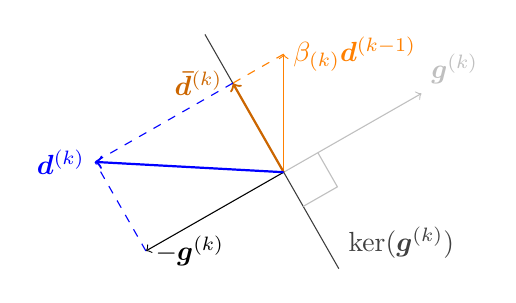
\begin{tikzpicture}
        \coordinate (origin) at (0,0);
        \coordinate (G0) at (origin);
        \coordinate (D0) at (G0);
        \coordinate (G1) at (1.75,1);
        \coordinate (D1) at (0.0, 1.5);
        \draw[->, lightgray] (G0) -- (G1) node[above right] {$\ve{g}\KK$};
        \draw[->] (G0) -- ($-1*(G1)$) node[right] {$-\ve{g}\KK$};
        \draw[->, orange] (D0) -- (D1) node[right] {$\beta\kK\vdKp$};

        \coordinate (P0) at ($(G0)!1.0!90:(G1)$);
        \coordinate (P1) at ($(G0)!-0.7!90:(G1)$);
        \draw[darkgray] (P1) node[above right] {$\orth(\ve{g}\KK)$} -- (P0);

        \coordinate (I) at ($(P0)!(D1)!(P1)$);
        \draw[dashed, orange] (D1) -- (I);
        \draw[->, orange!80!black, thick] (D0) -- (I) node[left] {$\ve{\bar{d}}\KK$};
    
        \pic [draw, lightgray, thin] {right angle = G1--G0--P1};

		\coordinate (D) at ($(I) - (G1)$);
		\draw[dashed, thin, blue] (I) -- (D);
		\draw[dashed, thin, blue] ($-1*(G1)$) -- (D);
		\draw[->, blue, thick] (G0) -- (D) node[left] {$\vdK$};
    \end{tikzpicture}
	\caption{
		Projection Scheme in the single-objective setting. The standard residual term is 
		projected onto the plane orthogonal to the gradient, so that the fincal \ac{cg}
		direction (blue) has sufficient decrease by construction.%
	}
\end{figure}

To go to the multi-objective setting, use the \ac{prp} coefficient
as in~\cite{lucambioperezNonlinearConjugateGradient2018}.
(If we used a coefficient similar to ~\eqref{eqn:factorialsPreemergent}
we would again need~\cref{ass:sublevelset_bounded} in the convergence proof.)
\begin{equation}
	\beta\kK = 
\frac{\funcXKp(\sdK) - \funcXK(\sdK)}{-\funcXKp(\sdKp)},
\quad
\kk\geq 1.
\label{eqn:tarnishesBandeaux}
\end{equation}
Moreover, for all $\kk \geq 1$, let $M\KK$ be a non-empty convex
subset of $\dCone(\vxK)$, containing the origin.
Lastly, define
\begin{equation}
	\vdK = 
	\begin{cases}
		\sdK
		&\text{if $\kk = 0$,}
		\\
		\sdK + \ve{\bar{d}}\KK
		&\text{if $\kk \geq 1$},
	\end{cases}
	\qquad
	\ve{\bar{d}}\KK 
	= 
	\proj{\beta\kK \vdKp}{M\KK}
	.
	\tag{PRP~MOII}
	\label{eqn:prpMOProj}
\end{equation}

\begin{remark*}
We can always use $M\KK = \dCone(\vxK)$, but then the projection
might be too expensive.
To exploit the single-vector projection formula from above, 
we can use a MiniMax approach, at least if $C$ is discrete.
Choose $\ve w^*$ as the minimizer in
$$
\min_{\ve w\in C}
\max_{\ve v\in C}
\mul{
	\ve v}{
	\jacf(\vxK)\proj{\beta\kK \vdKp}{\orth(\transp{\jacf(\vxK)}\ve w)}
}
$$
If the optimal at $\ve w$ is less than or equal to $0$,
then, by the properties of $\phiC$,
$$
\proj{\beta\kK \vdKp}{\orth(\transp{\jacf(\vxK)}\ve w^*)},
$$
a projection onto the hyperplane $\orth(\transp{\jacf(\vxK)}\ve w^*)$,
is contained in $\dCone(\vxK)$, and
we can use this as $\ve{\bar{d}}\KK$.
If the optimal value is positive, then $\beta\kK\vdKp$ belongs to
the polar cone of $\dCone(\vxK)$ and $\ve{\bar{d}}\KK = \vZ$
is the projection onto $\dCone(\vxK)$.
\end{remark*}

\begin{theorem}
The directions in~\eqref{eqn:prpMOProj} have the 
sufficient decrease property~\eqref{eqn:suff_dec}
with $\suffDecConst = 1$.
\end{theorem}
\begin{proof}
For $\kk=0$ the property is trivially satisfied.
Let $\kk\geq 1$.
As $\ve{\bar{d}}\KK$ is a projection onto $M\KK\subseteq \dCone(\vxK)$,
\begin{align*}
	\funcXK(\vdK)
	=
	\phiC(\jacf(\vxK)\args{\sdK + \ve{\bar{d}}\KK})
	\leq
	\phiC(\jacf(\vxK)\sdK)
	+ 
	\underbrace{\phiC(\jacf(\vxK)\ve{\bar{d}}\KK)}_{\leq 0}
	\leq 
	\funcXK(\sdK).
\end{align*}
\end{proof}

\begin{theorem}
	Suppose~\cref{%
	ass:funcs_differentiable,%
	ass:monotonic_seq_bounded}
	hold and that the criticality $\norm{\sdK}$ is 
	bounded below like in~\eqref{eqn:critBoundedBelow}.
	Then the Algorithm with modified Armijo-stepsizes
	according to~\eqref{eqn:armijo_strict} and with directions defined
	by~\eqref{eqn:prpMOProj} generates a critical subsequence.
\end{theorem}

\begin{proof}
	First, note that the projection onto a convex set is non-expansive.
	If the origin is contained in the convex set $M\KK$,
	then
	$$
	\norm{\proj{\ve v}{M\KK}} \leq \norm{\ve v}
	\qquad \forall \ve{v}\in \RRin.
	$$
	Let $\kk \geq 1$. We find that
	\begin{equation}	
	\norm{\vdK}
	=
	\norm{\sdK + \ve{\bar{\vd}}\KK}
	\leq
	\norm{\sdK} + 
	\norm{\ve{\bar{\vd}}\KK}
	\leq
	\norm{\sdK} + 
	|\beta\kK|
	\norm{\vd\KKp}.
	\label{eqn:stanchionsBotanizing}
	\end{equation}

	Per~\cref{ass:funcs_differentiable}, the Jacobian of $\vf$
	is Lipschitz.
	Suppose first that $\funcXKp(\sdK) \geq \funcXK(\sdK)$.
	Then
	\begin{align*}
	\norm{\funcXKp(\sdK) - \funcXK(\sdK)}
	&=
	{\funcXKp(\sdK) - \funcXK(\sdK)}
	\leq
	\phiC((\jacf(\vxKp) - \jacf(\vxK))\sdK)
	\\
	&\leq
	\Const_C \lipConstf \norm{\vxKp - \vxK} \norm{\sdK}
	=
	\Const_C \lipConstf \szKp \norm{\vdKp}\norm{\sdK},
	\end{align*}
	where the existence of $\Const_C>0$ follows from the 
	compactness of $\Const_C$.
	We find the same bound for the case $\funcXKp(\sdK) < \funcXK(\sdK)$.
	Looking at the definition~\eqref{eqn:tarnishesBandeaux}, 
	we see that there must be a constant $\Const_\beta > 0$ with
	$$
	|\beta\kK|
	\leq
	\frac{\Const_\beta
	\szKp \norm{\vdKp}\norm{\sdK}}
	{
		\norm{\sdKp}^2
	}.
	$$
	Combining this with~\eqref{eqn:stanchionsBotanizing} results in
	\begin{align}
		\frac{\norm{\vdK}}{\norm{\sdK}^2}
		&\leq
		\frac{1}{\norm{\sdK}}
		+
		\frac{
			\Const_\beta
			\szKp \norm{\vdKp}
		}{
			\norm{\sdK}
		}
		\frac{\norm{\vdKp}}{\norm{\sdKp}^2}
		\nonumber
		\\
		&\stackrel{\eqref{eqn:critBoundedBelow}}\leq
		\frac{1}{\critBound}
		+
		\frac{
			\Const_\beta
			\szKp \norm{\vdKp}
		}{
			\critBound
		}
		\frac{\norm{\vdKp}}{\norm{\sdKp}^2}
		.
		\label{eqn:pardiSubvocalisation}
	\end{align}
	Due to~\cref{thm:stepNorm_zero},
	the step-length goes to zero and there is a $\kk_0$ such that
	$\frac{
			\Const_\beta
			\szKp \norm{\vdKp}
		}{
			\critBound
		}<\mathtt{r}$
	for some $r\in (0,1)$ and all $\kk>\kk_0$.
	Analogous to the proof of~\cref{thm:prpMO1convergence},
	we can recurse~\eqref{eqn:pardiSubvocalisation} to deduce that $\frac{\norm{\vdK}}{\norm{\sdK}^2}$
	is uniformly bounded above for all $\kk\in\NN_0$,
	e.g., by $\mathtt A > 0$.
	Then
	$$
	\frac{\norm{\sdK}^4}{\norm{\vdK}^2}
	\geq \frac{1}{A^2} > 0
	\; \forall \kk \in \NN_0
	\quad\Rightarrow\quad
	\sum_{\kk\in\NN_0}
	\frac{\norm{\sdK}^4}{\norm{\vdK}^2}
	= 
	\infty,
	$$
	in contradiction to~\cref{thm:armijoZoutendijk}!
	Existence of a critical sequence follows by~\cref{thm:convergence}.
\end{proof}

\todo{Fix broken bibtex entries...}
% curl http://127.0.0.1:23119/better-bibtex/export/collection\?/1/2L27SBSD.bibtex -o refs.bib
\bibliography{refs}

\end{document}
